\documentclass[aspectratio=169,11pt]{beamer}

\usepackage{graphicx}
\usepackage{booktabs}

\graphicspath{{../results/robustness/}{../results/failures/}{../results/clean/}}

\usetheme{default}
\setbeamertemplate{navigation symbols}{}
\setbeamertemplate{itemize items}[circle]
\setbeamercolor{structure}{fg=blue!55!black}
\setbeamercolor{alerted text}{fg=orange!75!black}
\setbeamerfont{frametitle}{size=\large,series=\bfseries}
\setbeamertemplate{frametitle}{\vspace{4pt}\insertframetitle\vspace{-2pt}}
\setbeamertemplate{footline}{\hfill\scriptsize\insertframenumber\,/\,3\hspace{8pt}\vspace{3pt}}

\begin{document}

% ---------------------------------------------------------------- slide 1
\begin{frame}{Plant disease recognition when a robot takes the picture}
\footnotesize

\begin{columns}[T]
\begin{column}{0.56\textwidth}

\textbf{Task.} 38 plant disease classes, 14 crops, PlantVillage --- laboratory capture: one detached
leaf, uniform background, even light. 41\,275 / 10\,861 / 2\,169 images; the test split is carved by
\emph{moving} 5\,\% of each training class, so no leakage.

\vspace{6pt}
\textbf{Two transfer strategies}, one controlled variable --- which parameters get gradients:
\begin{itemize}
  \item \textcolor{blue!55!black}{\textbf{Frozen backbone}} --- linear probe, 77\,862 trainable parameters
  \item \textcolor{orange!75!black}{\textbf{Fine-tuned}} --- all 23\,585\,894 trainable
\end{itemize}

\vspace{6pt}
\textbf{Question.} A pretrained ResNet-50 saturates on clean PlantVillage, so the question is not
whether transfer works but \alert{which strategy survives leaving the laboratory}.

\vspace{4pt}
We model a field phenotyping robot: motion blur while driving, low light with sensor noise under the
canopy, JPEG compression for radio transmission --- three severities each, applied to the test set
only, no retraining.

\end{column}
\begin{column}{0.42\textwidth}
\centering
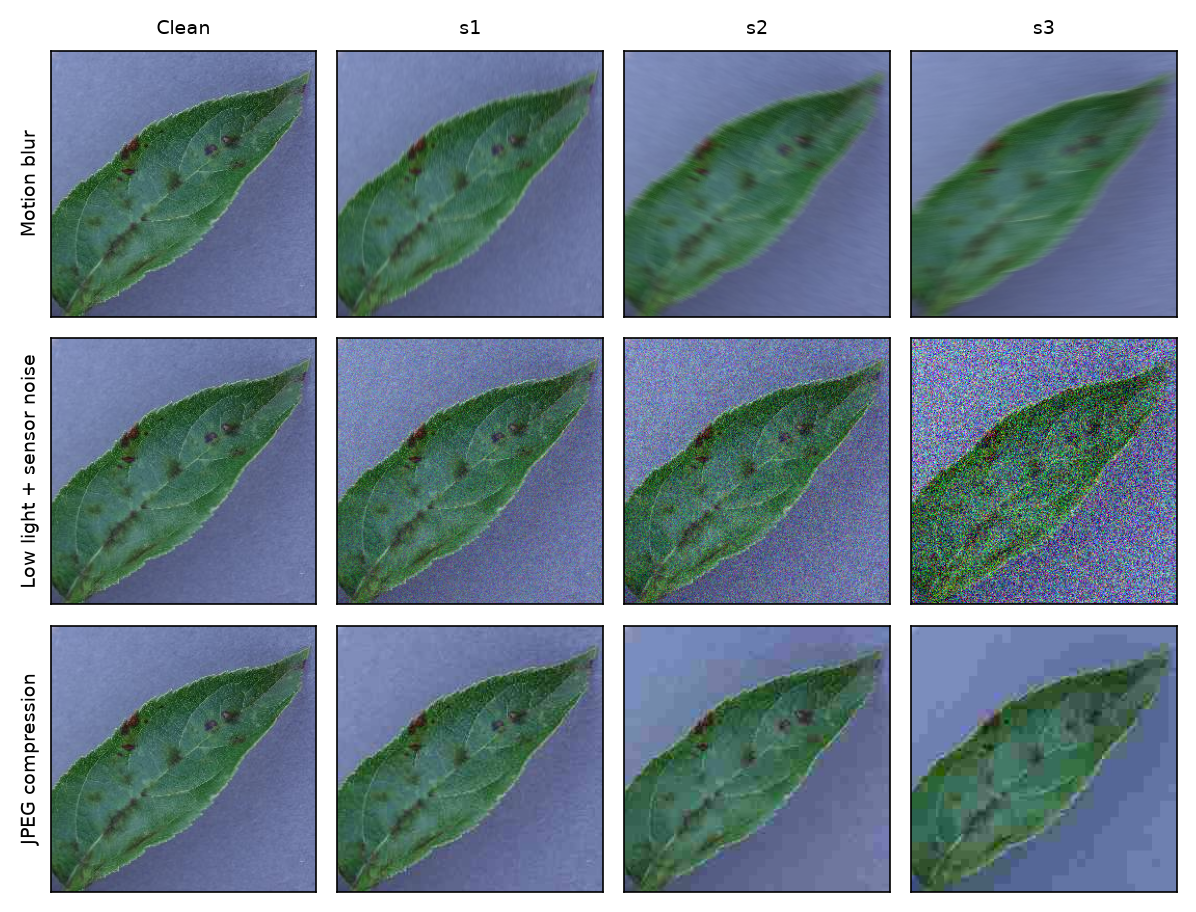
\includegraphics[width=\linewidth]{corruption_examples.png}

\vspace{2pt}
{\scriptsize Rows: motion blur, low light + noise, JPEG.\\
Columns: clean, then severity 1 to 3.}
\end{column}
\end{columns}
\end{frame}

% ---------------------------------------------------------------- slide 2
\begin{frame}{Clean data says one thing, degraded data says another}
\footnotesize

\begin{columns}[T]
\begin{column}{0.30\textwidth}
\centering
\begin{tabular}{@{}lrr@{}}
\toprule
Clean test & Froz. & F.-t. \\
\midrule
Accuracy & .970 & \textbf{.999} \\
Macro F1 & .966 & \textbf{.998} \\
Errors & 66 & \textbf{3} \\
\midrule
Train. params & 78\,k & 23.6\,M \\
Epochs & 47 & 16 \\
Time (min) & 14.7 & 9.9 \\
\bottomrule
\end{tabular}

\vspace{8pt}
\raggedright
Same graph, same parameter count $\Rightarrow$ identical inference cost: 4.74\,ms/image at batch 1,
0.31\,ms at batch 64, 773\,MB on an A100.

\vspace{6pt}
LR ablation $10^{-4}/10^{-3}/10^{-2}$: .9986 / .9991 / .9963 --- the comparison is not an artefact of
the learning rate.
\end{column}

\begin{column}{0.68\textwidth}
\centering
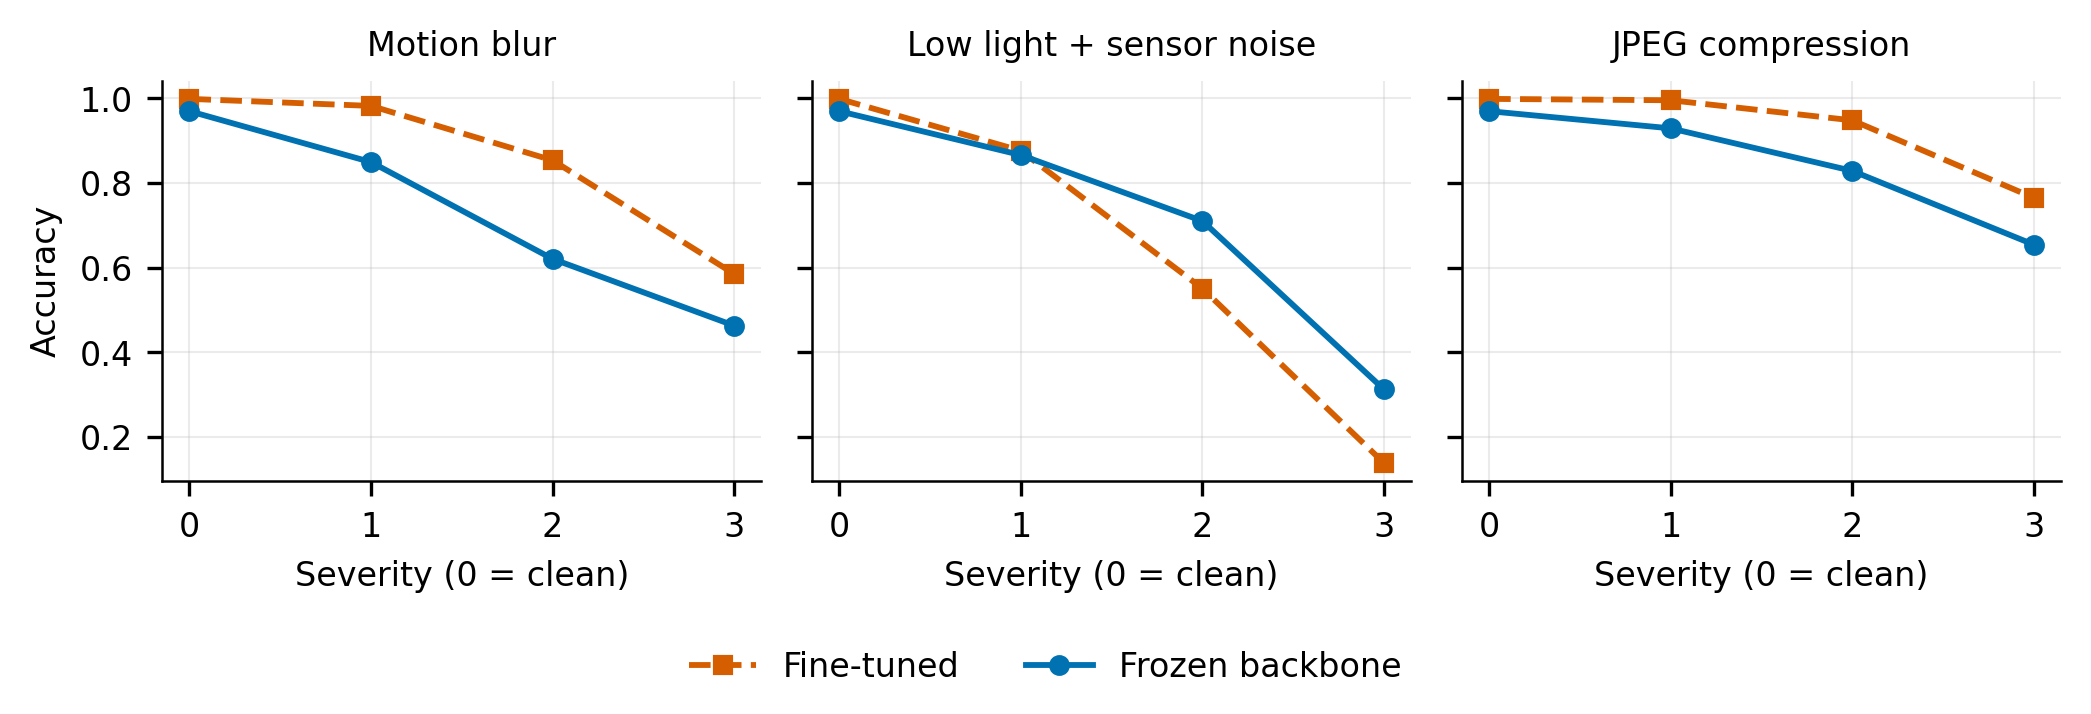
\includegraphics[width=\linewidth]{degradation_accuracy.png}

\raggedright
\vspace{2pt}
Fine-tuning wins under blur and JPEG at every severity, by up to 23 points. Under
\alert{low light with sensor noise the curves cross}: the frozen backbone is 16 points ahead at
severity 2 and 17 at severity 3.

\vspace{3pt}
Fine-tuning sharpens early filters onto the high-frequency statistics of noise-free laboratory
capture. Blur and JPEG \emph{remove} high frequencies; sensor noise \emph{injects} random energy into
exactly that band.
\end{column}
\end{columns}
\end{frame}

% ---------------------------------------------------------------- slide 3
\begin{frame}{What breaks, and what to take away}
\footnotesize

\begin{columns}[T]
\begin{column}{0.54\textwidth}

\textbf{Every clean error is a within-crop confusion} --- all 3 of the fine-tuned model and all 66 of
the frozen one. Cross-crop error rate: exactly zero. Corn Cercospora $\rightarrow$ Northern Leaf
Blight, Tomato Bacterial spot $\rightarrow$ Late blight, Target Spot $\leftrightarrow$ Spider mites.
The fine-tuned model's corn errors are leaves so far into necrosis that the distinguishing lesion
geometry is gone.

\vspace{6pt}
\textbf{Wrong, and confident about it.} Mean confidence on errors: 0.86 fine-tuned against 0.53
frozen. Under motion blur severity 3 it still reports 0.86 while being right 58.5\,\% of the time ---
it does not signal that it has left its operating regime.

\vspace{6pt}
\textbf{Fine-grained classes collapse first.} At low light severity 2 the fine-tuned model drops
Potato healthy, Cedar apple rust and Tomato Bacterial spot from F1 $\approx$ 1.0 to 0. ``No lesion''
becomes indistinguishable from ``lesion hidden by noise''.

\end{column}
\begin{column}{0.44\textwidth}

\textbf{Conclusion.}
\begin{itemize}
  \item Fine-tuning is the right default --- 3 errors against 66, in a third of the epochs.
  \item But robustness is \alert{artifact-dependent}: it is not a single number, and the ordering
        reverses under sensor noise.
  \item Pick the transfer strategy for the capture regime you expect, and report calibration, not
        only accuracy.
\end{itemize}

\vspace{8pt}
\textbf{Limitations.} Corruptions are simulated; focus, perspective and background are not modelled.
PlantVillage repeats the same physical leaf, so clean accuracy overstates generalisation. One
architecture, one dataset.

\vspace{8pt}
\scriptsize
\texttt{github.com/EgorSavchenko-web/} \\
\texttt{icv2026-plant-disease}

\end{column}
\end{columns}
\end{frame}

\end{document}
